%!TEX root = ../main.tex

\appendix

\section{A Learning-based Approach}
\label{sec:heuristic}
  
A drawback of the MILP approach is that the generated models grow with the 
size of the database and query log.
However, we argue that the encoded information is necessary in order to generate a sufficient set of constraints that result in a good repair.
In this section, we examine an alternative, simpler, decision tree-based approach called \dt. 
We show that even in a simple case of a single query log and a complete complaint set, it is expected to perform poorly.
We will first describe how to model the repair process using a decision tree,
and then we will present and discuss experimental results that illustrate its limitations.

\subsection{Modeling Repairs with Decision Trees}

Rule-based learners are used in classification tasks to generate a set of rules, or conjunctive predicates that best classify a group of labeled tuples.
The rules are non-overlapping, and each is associated with a label---a tuple that matches a given rule is assigned the corresponding label.
These rules exhibit a natural parallel with SQL \texttt{WHERE} clauses, 
which can be viewed as labeling selected tuples with a positive label and rejected tuples with a negative label.
Similarly, the structure of the rules is identical to those that \sys is designed to repair.
Thus, given the database tuples labeled to describe the errors, we may use a rule-based learner to
generate the most appropriate \texttt{WHERE} clause.
We focus our attention on rule-based learners;
specifically, we experiment with the C4.5~\cite{quinlan1987} decision tree learner, which is an 
exemplar of rule-based learners.

A core limitation of this classification-based approach is that there is no means to 
repair \texttt{SET} clauses, which modify data values rather than simply label them.
We resolve this with a two step approach.
We first use the decision tree to generate a repair for the
\texttt{WHERE} clause, and then use the modified query to identify repairs for the \texttt{SET} clause.
The need for this two step procedure limits this approach to encoding and repairing at most one query
at a time.

\noindent
\textbf{Repairing the WHERE Clause:}
The \texttt{WHERE} clause of an update query is equivalent to a
rule-based binary classifier that splits tuples into two groups:
(1)~tuples that satisfy the conditions in the \texttt{WHERE} clause
and (2)~tuples that do not. A mistake in a query predicate can 
cause a subset of the tuples to be misclassified, and in turn,
translate into data errors. 
Therefore, repairing the complaints corresponds to repairing the imprecise classification. 

The repair works as follows: For an incorrect query $q$, let
$D_0$ be the database state before $q$, and $D_1^*$ the \emph{correct}
database state that should have been the result after $q$, if $q$ were correct.
We use each tuple $t \in D_0$ as an element in the input training data
for the classifier where the values (of each attribute) of $t$ define
the feature vector and the label for $t$:
	\[
    label(t)= 
    \begin{cases}
    true & \textrm{if\ }D_0.t \neq D_1^*.t\\
    false              & \text{otherwise}
    \end{cases}
\]
The \texttt{true} rules generated by the decision tree trained on this labeled dataset 
forms a disjunction of rules that constitute the repaired \texttt{WHERE} clause.


\noindent
\textbf{Repairing the SET Clause:}
The \texttt{WHERE} clause repair proposed by the classifier may not completely repair 
the complaints if there was also an error in the \texttt{SET} clause. 
In this case, we execute a second repair step.
\begin{figure}[t]
\centering
  \begin{subfigure} [t]{.75\columnwidth}
  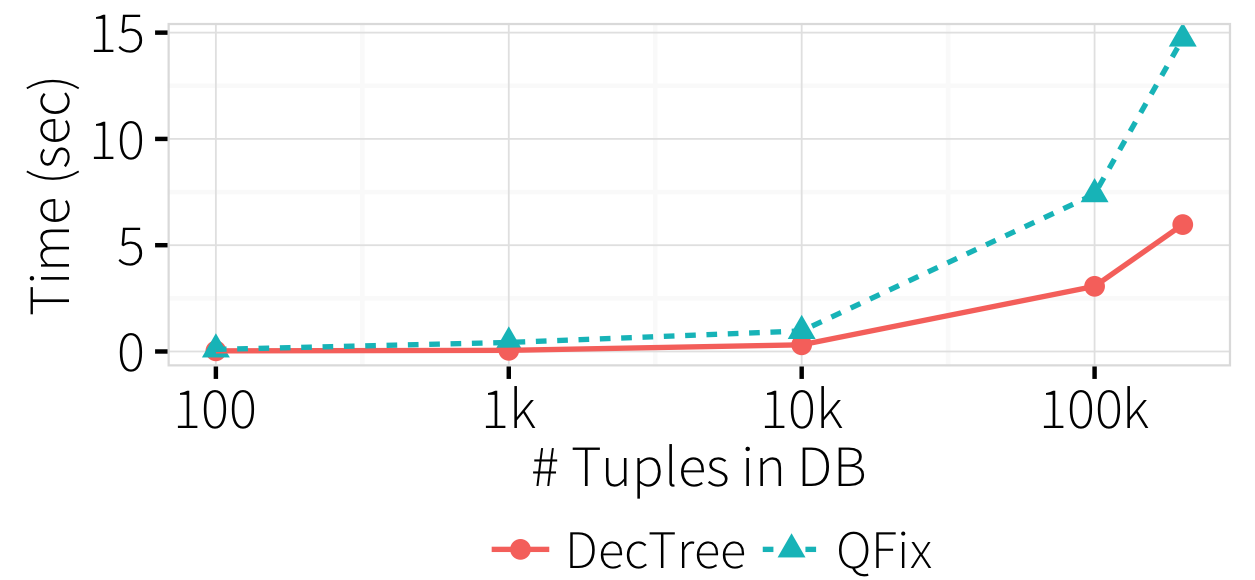
\includegraphics[width = \columnwidth]{figures/heuristictime}
  \caption{Comparison on Performance.}
  \label{f:heuristic_time} 
  \end{subfigure}\\

  \begin{subfigure} [t]{.75\columnwidth}
  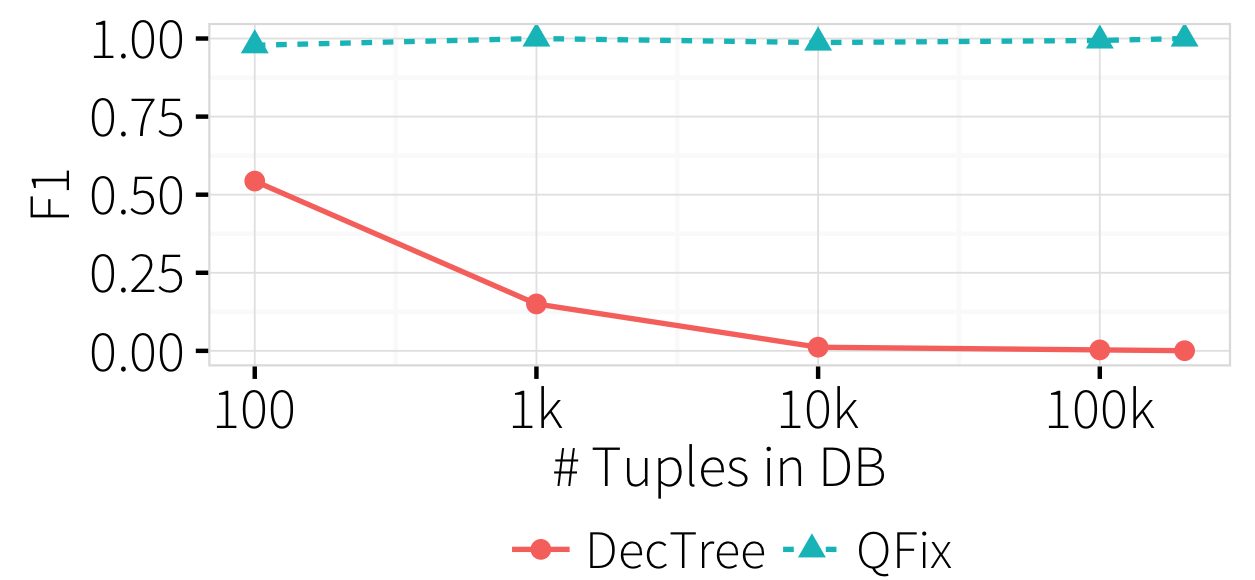
\includegraphics[width = \columnwidth]{figures/heuristicacc}
  \caption{Comparison on Accuracy.}
  \label{f:heuristic_acc} 
  \end{subfigure}
 \caption{\dt compared with \sys}
 \label{f:heuristic}
\end{figure}


We model the errors as a simple linear system of equations: 
each expression in the \texttt{SET} clause is translated into a
linear equation in the same fashion as described in Section~\ref{sec:sol}.
Directly solving the system of equations for the undetermined variables 
will generate the desired repair for the \texttt{SET} expression.



\subsection{Experimental Results}

To illustrate these shortcomings, we compare \dt with \sys using a simplified version of the setup from Section~\ref{sec:experiments} that favors \dt.
We restrict the query log to contain a single query that is corrupted, use a complete complaint set  and vary the database size.
We use the following query template, where all \texttt{SET} clauses assign the attributes to constants,
and the \texttt{WHERE} clauses consist of range predicates:

{\scriptsize
\begin{verbatim}
  UPDATE table
  SET  (a_i=?), ...
  WHERE a_j in [?,?+r] AND ...
\end{verbatim}
}

Figure~\ref{f:heuristic_time} shows that although the runtime performance of \dt is better than \sys by small a constant factor ($\sim 2.5 \times$),
both runtimes degrade exponentially.
In addition, the \dt repairs are effectively unusable as their accuracy is low: the F1-score starts at $0.5$ and rapidly degrades towards $0$.
From these empirical results, we find that \dt generates low-quality repairs even under the simplest conditions---an approach
that applies \dt over more queries is expected to have little hope of succeeding.



There are three important reasons why \dt, and any approach that focuses on a single query at a 
time\footnote{Although our incremental approach tries to generate a repair for a single query at a time, it encodes all subsequent queries in the log.}, will not perform well.

\begin{itemize}[itemsep=1pt, leftmargin=5mm]
\item \textbf{Single Query Limitation: }
In principle, one could attempt to apply this technique to the
entire log one query at a time, starting from the most recent query.
Even ignoring the low repair accuracy shown in Figure~\ref{f:heuristic_acc},
this approach is infeasible.
Consider that we generate a labeled training dataset to repair $q_i$ 
using the query's input and output database states $D_{i-1}$ and $D_i^*$.
Note that $D_i^*$ is the theoretically \emph{correct} database state assuming no errors in the query log.
We would need to derive $D_i^*$ by applying the complaint set to $D_n$ to create $D_n^*$, and roll back the database state.
Unfortunately, \texttt{UPDATE} queries are commonly surjective such
that their inverses are ambiguous, which means that it is often
impossible to derive $D_i^*$. In contrast, the incremental version of
\sys can bypass this problem by encoding subsequent queries in the log
in a MILP representation.


\item \textbf{Structurally Different \texttt{WHERE} Clause Results: } 
The basic classifier approach simply learns a set of rules to minimize
classification error, and can derive a clause whose struture is arbitrarily 
different from the original query's \texttt{WHERE} clause.
Although it may be possible to incorporate a distance measure as part of the decision tree
splitting criteria, it is likely to be a heuristic with no guarantees.


\item \textbf{High Selectivity, Low Precision: }
Classifiers try to avoid overfitting by balancing the complexity of the rules with classification accuracy.
This is problematic for highly selective queries (e.g., primary key updates), because the classifier
may simply ignore the single incorrect record and generate a rule such as \texttt{FALSE}.
In fact, this form of severely imbalanced data continues to be a challenge for most major classification algorithms~\cite{he2009learning, galar2012review}. 
Thus, we believe that alternative classification algorithms would not improve on these results. 
Compound with the fact that many workloads are primarily composed of
key update queries~\cite{oltpbench} this issue severely limits the
applicability of learning-based approaches.

\end{itemize}


\section{Repairing the Correct Query}
\label{app:index}


Our experiments in Section~\ref{sec:experiments} measure the accuracy of \sys
based on the effect of the repairs to the dataset. However, it is possible to
correctly resolve the reported complaints by modifying a query that was not
corrupted. Here we augment our evaluation to study how often \sys chooses the
right query to repair.  For each setting, we compute the \emph{correct repair
ratio} $p_{correct}$ over 20 runs: $p_{correct}$ is the portion of runs where \sys
chose the correct query to repair.

In Figure~\ref{f:querytyperatio}, we evaluate \qfix with three types of
workloads (\texttt{UPDATE}, \texttt{INSERT}, and \texttt{DELETE}) over
increasing corruption age: corruption age 1 means that the most recent query
was corrupted, while corruption age 250 means that the corruption occurred 250
queries in the past. In this experiment, we assume complete knowledge of the
complaint set. \sys selects the correct query to repair in all cases. We next
focus on the \texttt{UPDATE} workload and three ages of corruption, while
increasing the database size. Again, \sys is accurate in every case
(Figure~\ref{f:dbsizeratio}).

   \begin{figure*}[t]
  \centering
  \begin{subfigure} [t]{.3\textwidth}
    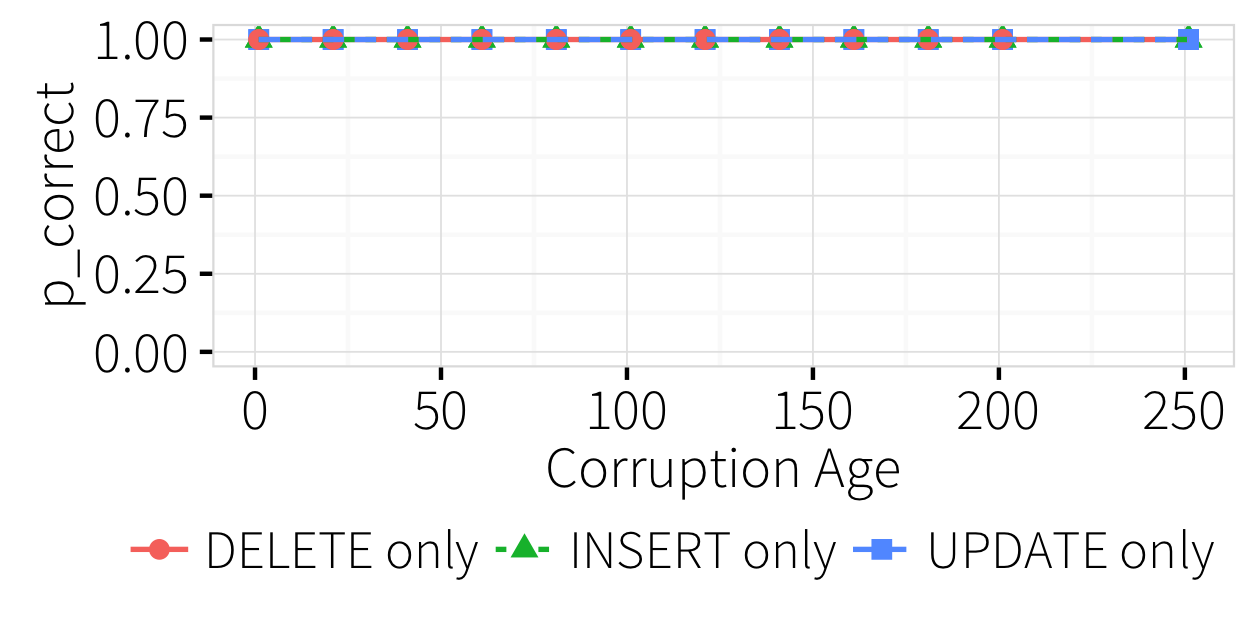
\includegraphics[width = .99\columnwidth]{figures/indelup_acc_idx}
    \vspace*{-.25in}
    \caption{Correct repair ratio vs. query types}
    \label{f:querytyperatio} 
    \end{subfigure}
    \begin{subfigure} [t]{.3\textwidth}
    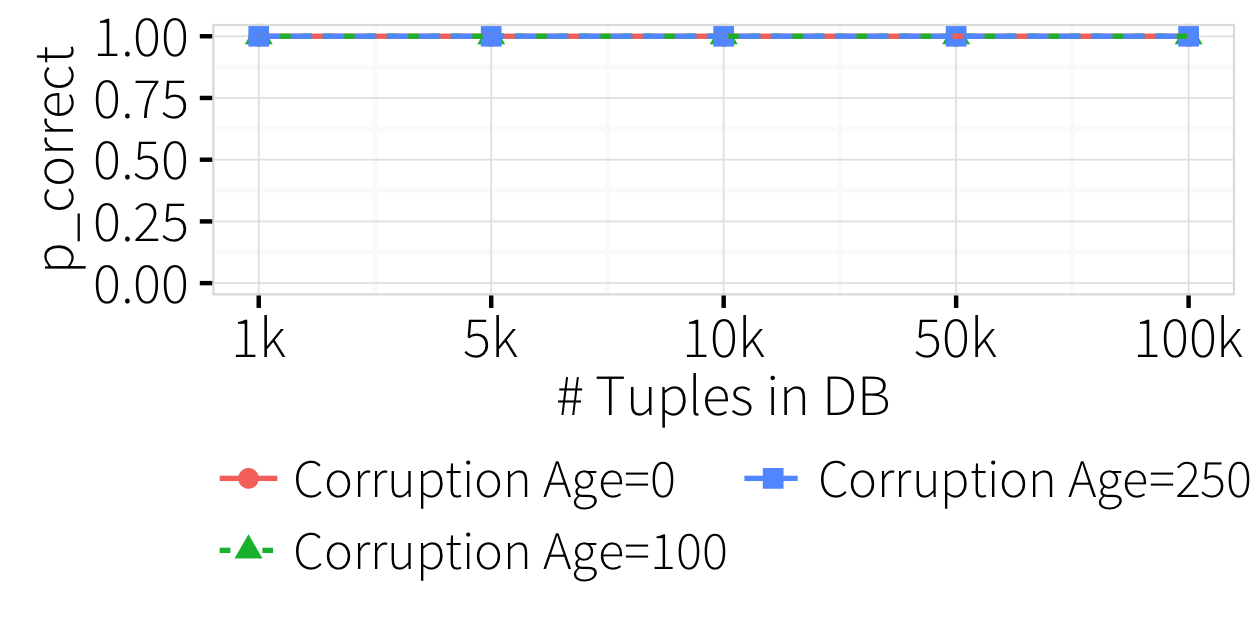
\includegraphics[width = .99\columnwidth]{figures/dbsize_acc_idx}
    \vspace*{-.25in}
    \caption{Correct repair ratio vs. database sizes}
    \label{f:dbsizeratio} 
    \end{subfigure}
    \begin{subfigure} [t]{.3\textwidth}
    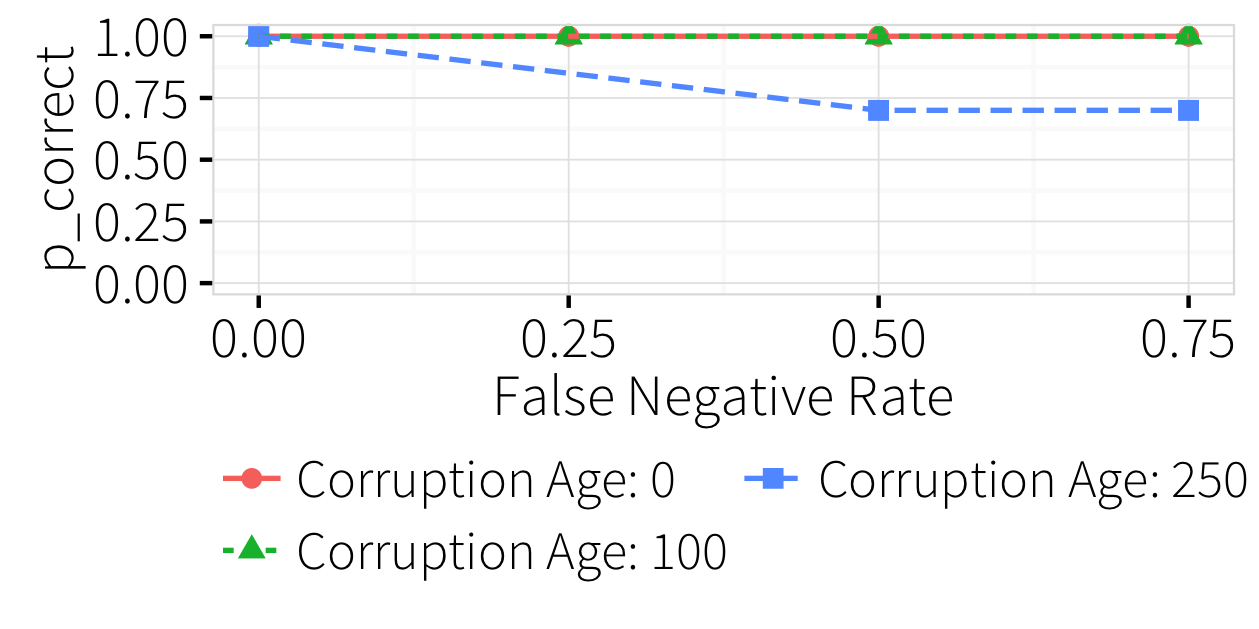
\includegraphics[width = .99\columnwidth]{figures/noise_fn_acc_idx}
    \vspace*{-.25in}
    \caption{Top-k vs. query types. }
    \vspace*{-.1in}
    \label{f:noiseratio} 
    \end{subfigure}
   \caption{ \sys maintains 1.0 correct repair ratio with complete complaint set. }
   \vspace*{-.1in}
   \label{fig:truerate}
  \end{figure*}

Finally, we study the effect of incomplete complaints in
Figure~\ref{f:noiseratio}. Increasing the false negative rate means that more
complaints are not reported. Similar to the precision and recall performance
in Figure~\ref{f:falsenegative_acc}, $p_{correct}$ also drops for problems
with old corruptions and high false negative rates. This is expected since
with insufficient information, there is a larger number of queries that offer
valid fixes and \sys simply chooses the one with the lowest objective. 






% \subsection{Experimental Results}
% To evaluate \sys's ability in identifying the correct query to fix, we summarize our results using \textit{Correct repair ratio}, $p_{correct}$, which is the number fixes on the true query divided by total number of runs.
% 
% \textbf{Complete Complaint Set: } We first evaluate three types of workloads with increasing corruption age. The database is set to the default setting and conclude the average $p_{correct}$ across 20 random runs. In Figure~\ref{f:querytyperatio}, we first evaluate $p_{correct}$ rate on three types of workloads: \sys identifies the correct query to fix ($p_{correct} = 1.0$) for all three types of workloads, \texttt{UPDATE},  \texttt{INSERT}, and \texttt{DELETE} workloads. We next narrow down to \texttt{UPDATE} workload and evaluate \sys's behavior with increasing amount of tuples in the database. We observe $p_{correct} = 1$ on different corrupt indexes in all database sizes (Figure~\ref{f:dbsizeratio}). 
% 
% \textbf{Incomplete Complaint Set: } In Figure~\ref{f:noiseratio}, we study the performance of \sys with increasing false negative rate in the incomplete complaint set. Similar to the precision and recall performance in Figure~\ref{f:falsenegative_acc}, $p_{correct}$ also drops for problems with old corrupted query and high false negative rate. This is expected since with insufficient information, \sys tends to fix the wrong query with better objective function value as long as all the reported errors are all resolved. 


\section{Query Interactions} \label{app:selectivity}

\begin{figure}[t]
\centering
  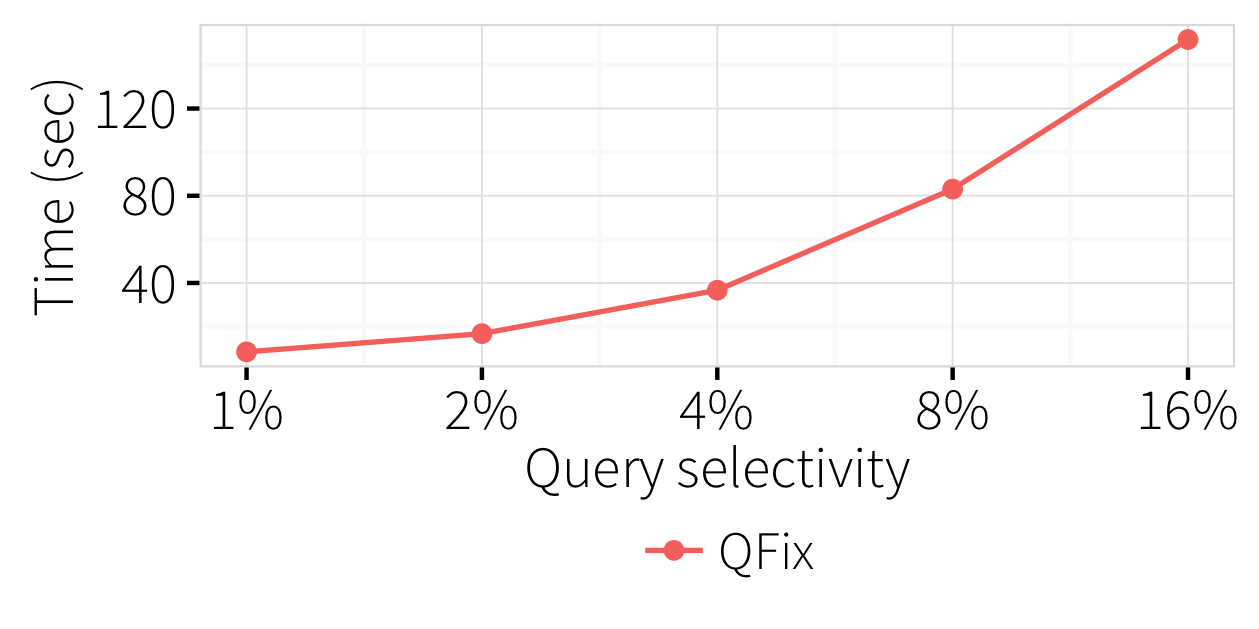
\includegraphics[width =.75\columnwidth]{figures/rangevstime}
 \caption{ Increasing query selectivity leads to longer \sys execution time.}
  \label{f:selectivityvstime} 
\end{figure}

One of the challenges that motivates our work on \sys is that the progression
of queries in the log obscures and propagates errors, as subsequent queries
interact with tuples affected by a prior erroneous query. Our synthetic data
generator (Section~\ref{sec:setup}) does not directly control the degree of
interaction among queries in the log, but parameters such as the number of
attributes and the dataset size impact this directly. Here we compute the
probability that any two tuples in the log interact, through the random
generation process. We assume two \texttt{UPDATE} queries, $q_i$ and $q_j$,
with range \texttt{WHERE} predicates.  The probability that $q_i$ and $q_j$ interact (i.e., the intersection of the tuples they update is non-empty) is:
\begin{multline*}
Pr(q_i\cap q_j \neq \emptyset) =\\ 
Pr(\sigma_{q_i}.A= \sigma_{q_j}.A)Pr(q_i\cap q_j \neq \emptyset |\sigma_{q_i}.A= \sigma_{q_j}.A) \\
+ Pr(\sigma_{q_i}.A\neq \sigma_{q_j}.A)Pr(q_i\cap q_j \neq \emptyset |\sigma_{q_i}.A\neq \sigma_{q_j}.A), 
\end{multline*}



Here, $Pr(\sigma_{q_i}.A= \sigma_{q_j}.A)$ is the probability that the
\texttt{WHERE} clauses of the two queries have predicates on the same
attribute; $Pr(\sigma_{q_i}.A= \sigma_{q_j}.A)=\frac{1}{N_a}$, where $N_a$ is
the number of attributes in the database. The probability that the
\texttt{WHERE} clause ranges of the two queries intersect is $Pr(q_i\cap q_j
\neq \emptyset |\sigma_{q_i}.A= \sigma_{q_j}.A) = 2*s$, where $s$ is the
predicate selectivity. Similarly for the second term, $Pr(\sigma_{q_i}.A\neq
\sigma_{q_j}.A) = \frac{N_a-1}{N_a}$ is the probability that the
\texttt{WHERE} clauses of $q_i$ and $q_j$ use different attributes. Assuming
tuple values are evenly distributed, the number of tuples selected by each
query is roughly $n = N_d \cdot s$, where $N_d$ is the number of tuples in the
database. Thus, the probability that these two queries update at least one
common tuple is $Pr(q_i\cap q_j \neq \emptyset |\sigma_{q_i}.A\neq
\sigma_{q_j}.A) = 1 - \frac{C(N_d - n, n)}{C(N_d, n)}$, where $C$ computes the
combinations $C(n,r) = \frac{n!}{r!(n-r)!}$. Therefore, the probability that
two queries in our dataset interact is:
\begin{multline} \label{eq:pr}
Pr(q_i\cap q_j \neq \emptyset) = \frac{2s}{N_a} + \frac{N_a-1}{N_a} \cdot (1 - \frac{C(N_d - n, n)}{C(N_d, n)}), 
\end{multline}
Where $n = N_d \cdot s$. Based on this result, the probability that any two
queries interact with each other with the default parameter settings of our
generator is about $0.31$.

In Section~\ref{sec:experiments:dbproperties}, we study the influence of the
number of attributes $N_a$ on \sys performance (Figure~\ref{f:attr}) and
observe that more attributes result in faster execution time with all
optimizations. This is expected as $Pr(q_i\cap q_j \neq \emptyset)$ is
inversely proportional to the number of attributes, which means that there are
fewer interactions. Therefore, fewer interactions lead to faster runtimes.

We also evaluate \sys over different query selectivities. In
Figure~\ref{f:selectivityvstime}, we observe that the execution time of \sys
increases with higher query selectivity, which results in higher query
interaction.


%%%%%%%%%%%% %%%%%%%%%%%%%%
%%%%%%%%%% the end %%%%%%%%%%%%
%%%%%%%%%%%% %%%%%%%%%%%%%%

\iffalse


\section{MILP Solver Performance}
\label{app:solvtime}

Some background about why we are runnig these experiments.  What is known about MILP solvers already.

\subsection{Factors Relevant to Solver Performance}

\iffalse
  \begin{figure*}[t]
  \centering
      \begin{subfigure} [t]{.3\textwidth}
    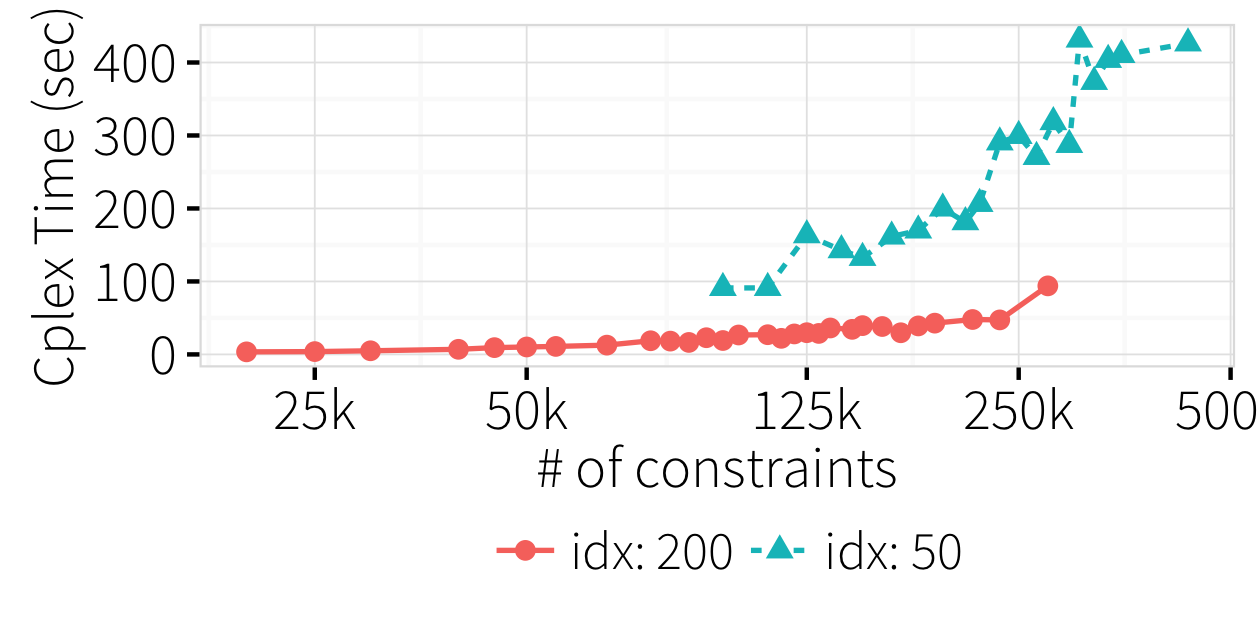
\includegraphics[width = .99\columnwidth]{figures/num_cons_time}
    \vspace*{-.25in}
    \caption{\# of constraints vs. solver solving time.}
    \vspace*{-.1in}
    \label{f:cons_vs_time} 
    \end{subfigure}
    \begin{subfigure} [t]{.3\textwidth}
    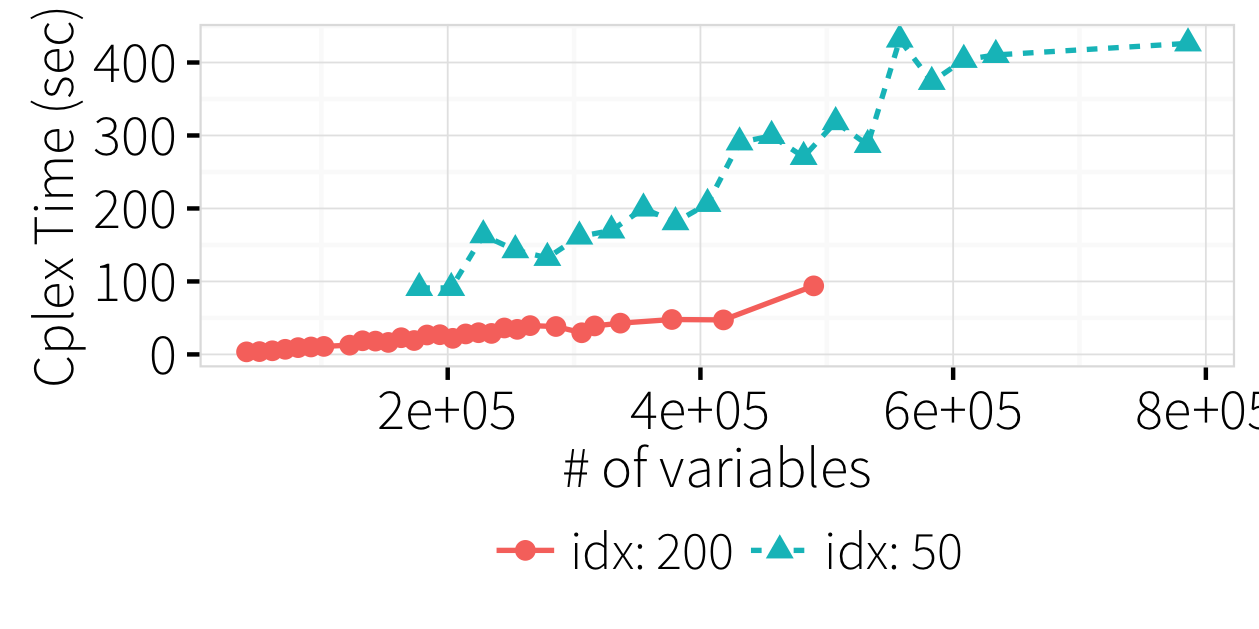
\includegraphics[width = .99\columnwidth]{figures/num_vars_time}
    \vspace*{-.25in}
    \caption{\# of undetermined variables vs. solver solving time.}
    \vspace*{-.1in}
    \label{f:var_vs_time} 
    \end{subfigure}
    \begin{subfigure} [t]{.3\textwidth}
    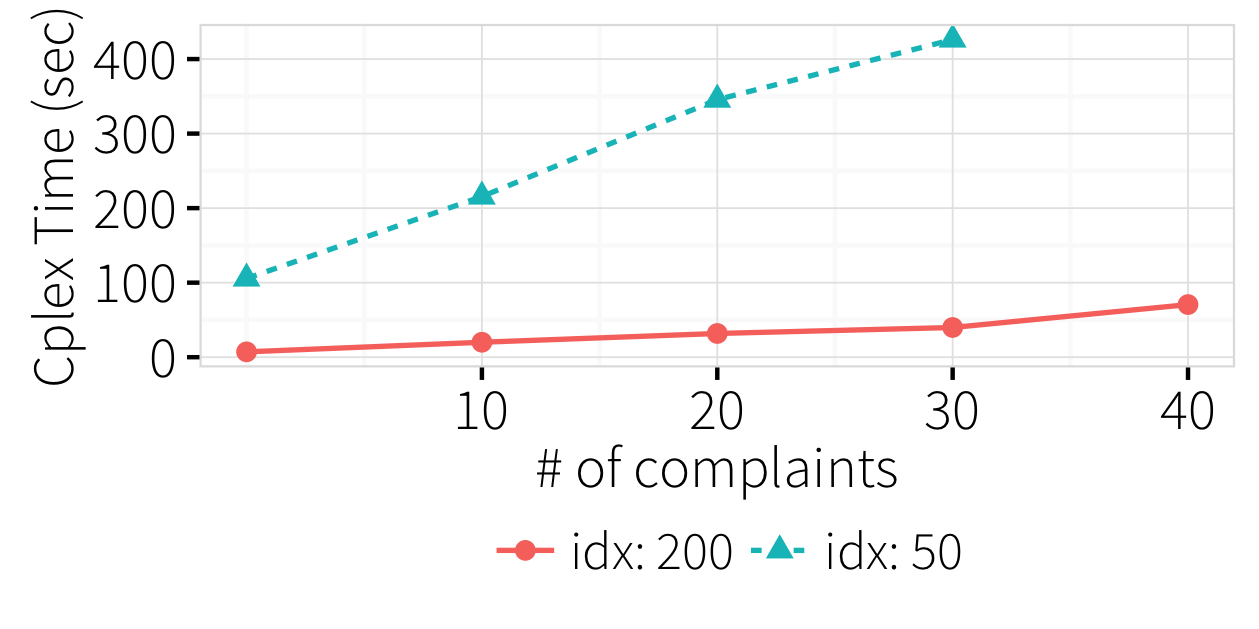
\includegraphics[width = .99\columnwidth]{figures/num_compl_time}
    \vspace*{-.25in}
    \caption{\# of compl. vs. solver solving time.}
    \vspace*{-.1in}
    \label{f:compl_vs_time} 
    \end{subfigure} 
    \iffalse
    \begin{subfigure} [t]{.3\textwidth}
    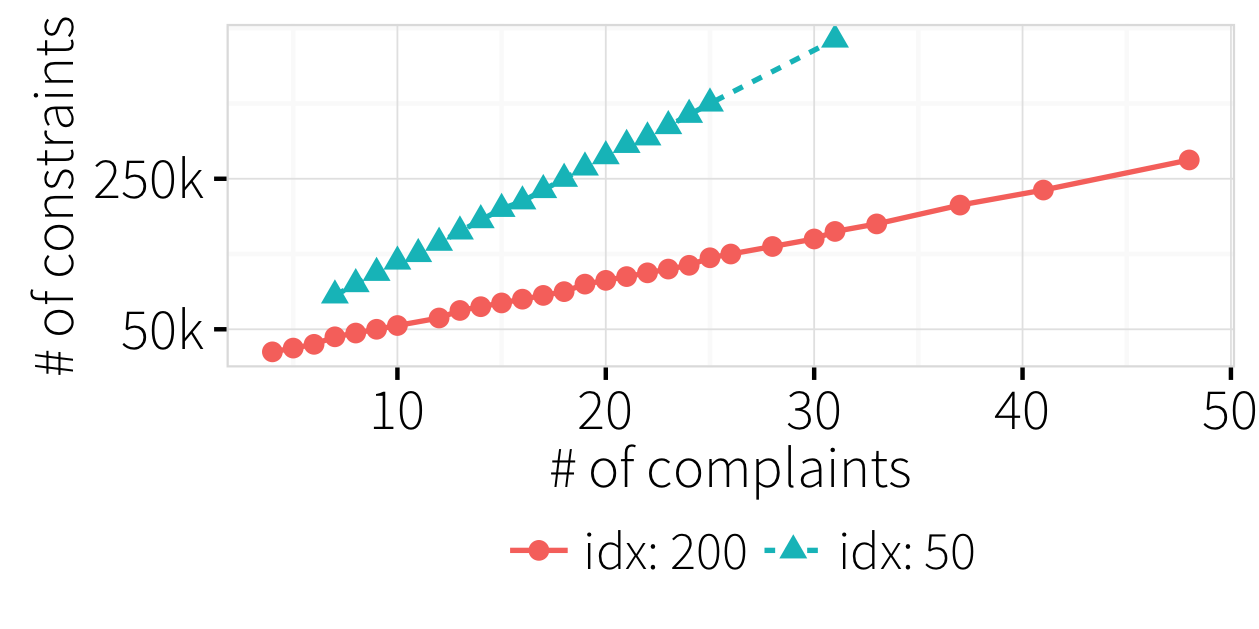
\includegraphics[width = .99\columnwidth]{figures/num_compl_cons}
    \vspace*{-.25in}
    \caption{\# of constraints vs.\# of compl.}
    \vspace*{-.1in}
    \label{f:compl_vs_cons} 
    \end{subfigure}
    \begin{subfigure} [t]{.3\textwidth}
    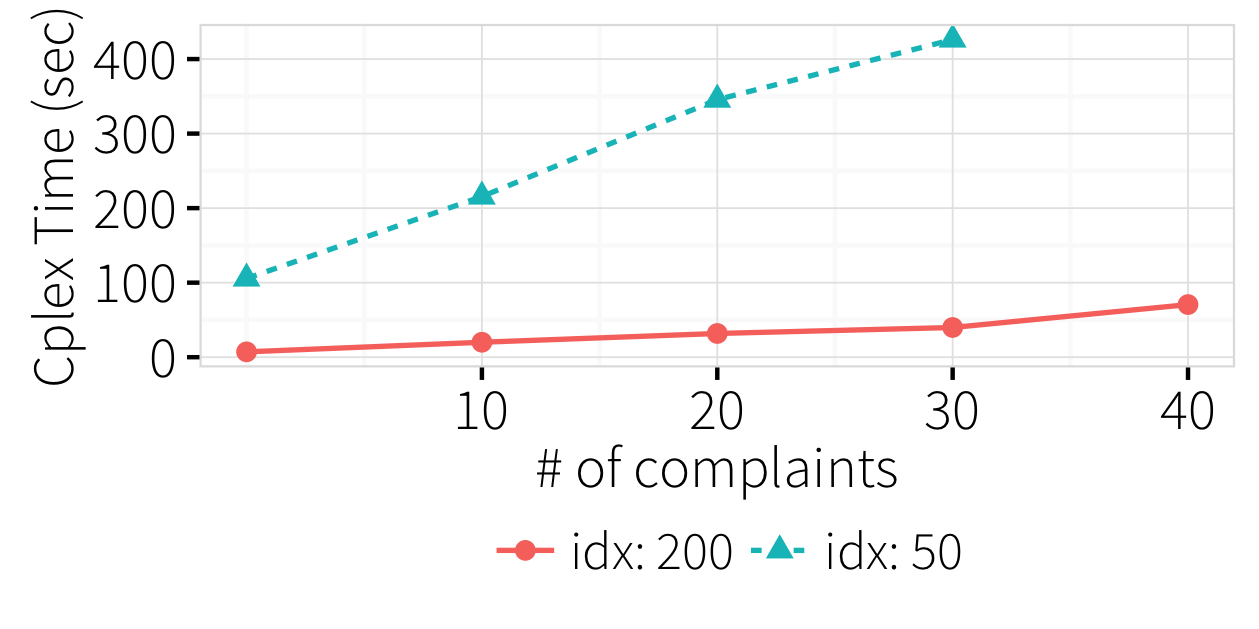
\includegraphics[width = .99\columnwidth]{figures/num_compl_time}
    \vspace*{-.25in}
    \caption{\# of undetermined variables vs. \# of compl.}
    \vspace*{-.1in}
    \label{f:compl_vs_time}
    \end{subfigure}
    \fi
   \caption{Solver solving time grows with all three factors: number of constraints, number of undermined variables and number of complaints. }
   \vspace*{-.1in}
   \label{f:soltime}
  \end{figure*}
\fi
\ewu{reference other constraint performance papers}
In this section, we study factors that influence the MILP solver solving time. In this paper, we
use IBM CPLEX~\cite{cplex2014v12} as a black box to solve the constructed MILP problems.  \ewu{describe MILP problems to justify why we focus on num constraints and num variables.} Similar to many solver performance studies~\cite{atamturk2005integer, meindl2012analysis, gearhart2013comparison}, 
we majorly study the connection between solver performance between \textit{the number of constraints} and \textit{the number of variables} in the constructed MILP problem. For this, we create \texttt{UPDATE}-only workloads using our synthetic data generator for 300 queries with constant \texttt{SET} clause and range \texttt{WHERE} clause: 

{\scriptsize
\begin{verbatim}
  UPDATE table
  SET  (a_i=?), ...
  WHERE a_j in [?,?+r] AND ...
\end{verbatim}
}
We further corrupt two query indexes, $q_{50}$ and $q_{200}$, to create the dirty query logs. \xlw{We only show results for  \texttt{UPDATE}-only workloads since all types of workloads show similar correlations. In addition, the selected corrupt query indexes allow us to evaluate the solver performance over median to large problem sizes.}  \ewu{We chose these because...} 


\smallskip
\emph{Number of Constraints: } We first study the relationship between solver performance and number of constraints. \xlw{The number of constraints is controlled via multiple factors including the number of complaints, corrupt query index, complexity of queries. Due to the randomness in synthetic data generator, we are not able to control the size of constraints to a specific value.} \ewu{Explain that the number of constraints is not controlled by you, which is why the lines start and end at different values in the figures.} From Figure~\ref{f:cons_vs_time}, we observe that solver time is roughly positive proportional, with tiny fluctuation, to the number of constraints in both corrupt indexes. This is expected because increasing the number of constraints by large scale usually accompany with significantly greater amount of variables in the MILP problem, which lead to harder MILP problems by natural. However, MILP problems \ewu{cite MILP papers that say this, so it's clear we are describing well known problems} with slightly larger amount of constraints sometimes could be even easier to solve since the additional constraints help pruning the searching space for similar amount of variables.

\smallskip
\emph{Number of Variables: } Similar to the previous experiment, we next compare the solver time with the number of variables. As shown in Figure~\ref{f:var_vs_time}, we find highly correlated trends compare to Figure~\ref{f:cons_vs_time}. 
This is due to the way we construct the MILP problem: the number of constraints and the number of variables grows linearly with \textit{the number of queries and the number complaints}.  



\iffalse
 In our experiments we found that increasing the number of constraints by increasing the database, query log, or complaint set sizes aversely affects the solver performance,
  solver performance has been shown to \emph{improve} as constraints that effectively reduce the problem space are added to the problem.  
  Thus, we now focus on the effects on the number of undetermined variables, which strictly increases the problem space.
  We keep the number of constraints fixed, however increase the number of undetermined variables by \ewu{XL fill in}. \xlw{need to rerun exp to get required numbers. We need to gradually increase the batch size to achieve this. }

\fi

In Figure~\ref{f:compl_vs_time} we illustrate the above argument by comparing the average solver time between the number of complaints at two different corrupt indexes. This allows us to study the relationship between solver time with both the number of complaints (x-axis) and the number of queries (two indexes). As expected, with the same number of complaints, the solver solving time for corrupt index $50$ is significantly higher than index $200$ since the number of queries encoded in each problem is $250$ and $100$ respectively. In contrast, with the same corrupt query index, problems with higher amount of complaints has much higher average solver solving cost than problems with lower amount of complaints. We believe that this is because increasing the number of queries and the number of complaints would increase both the number of variables and constraints in the constructed MILP problem. 

\xlw{The number of variables and constraints are two quantifiable factors that influence the solver time in solving MILP problems. However, there are other non-quantifiable factors, including but not limited to the correlations among variables, searching space of under-determined variables after pre-processing, that also relevant to the hardness of the MILP problem, which determines the solver time. These non-quantifiable factors are hard to control and optimize. Thus, in this paper, we mainly focus on optimizing (reducing) the quantifiable factors -- number of variables and constraints in order to reduce the  solver time. }

\subsection{Factors Relevant to the Number of Complaints}

From the above experiments, we observe that the solver time is highly correlated to the number of complaints and the number of queries we encoded in a MILP problem. The number of queries can be easily controlled by a particular parameter $N_q$. The number of complaints, on the other hand, is a reflection of the queries that have run over the database. It is influenced by  factors including the \texttt{SET} clause type, corrupt query index, query skewness, \texttt{WHERE} clause range, and some random factors. \ewu{however, don't know how the affect the complaint set.}  To better understand factors that control the size of the complaint set, we ran simulations using a database with $20$ attributes, and a query log of size $1000$ containing
either all constant or relative \texttt{SET} clause \texttt{UPDATE} queries. We found that SET and relative queries behave differently.
We varied the number of corrupt index uniformly throughout the query log, and additionally varied
the skew and range parameters to study how they affect the size of the complaint sets.



\begin{figure}[t]
\centering
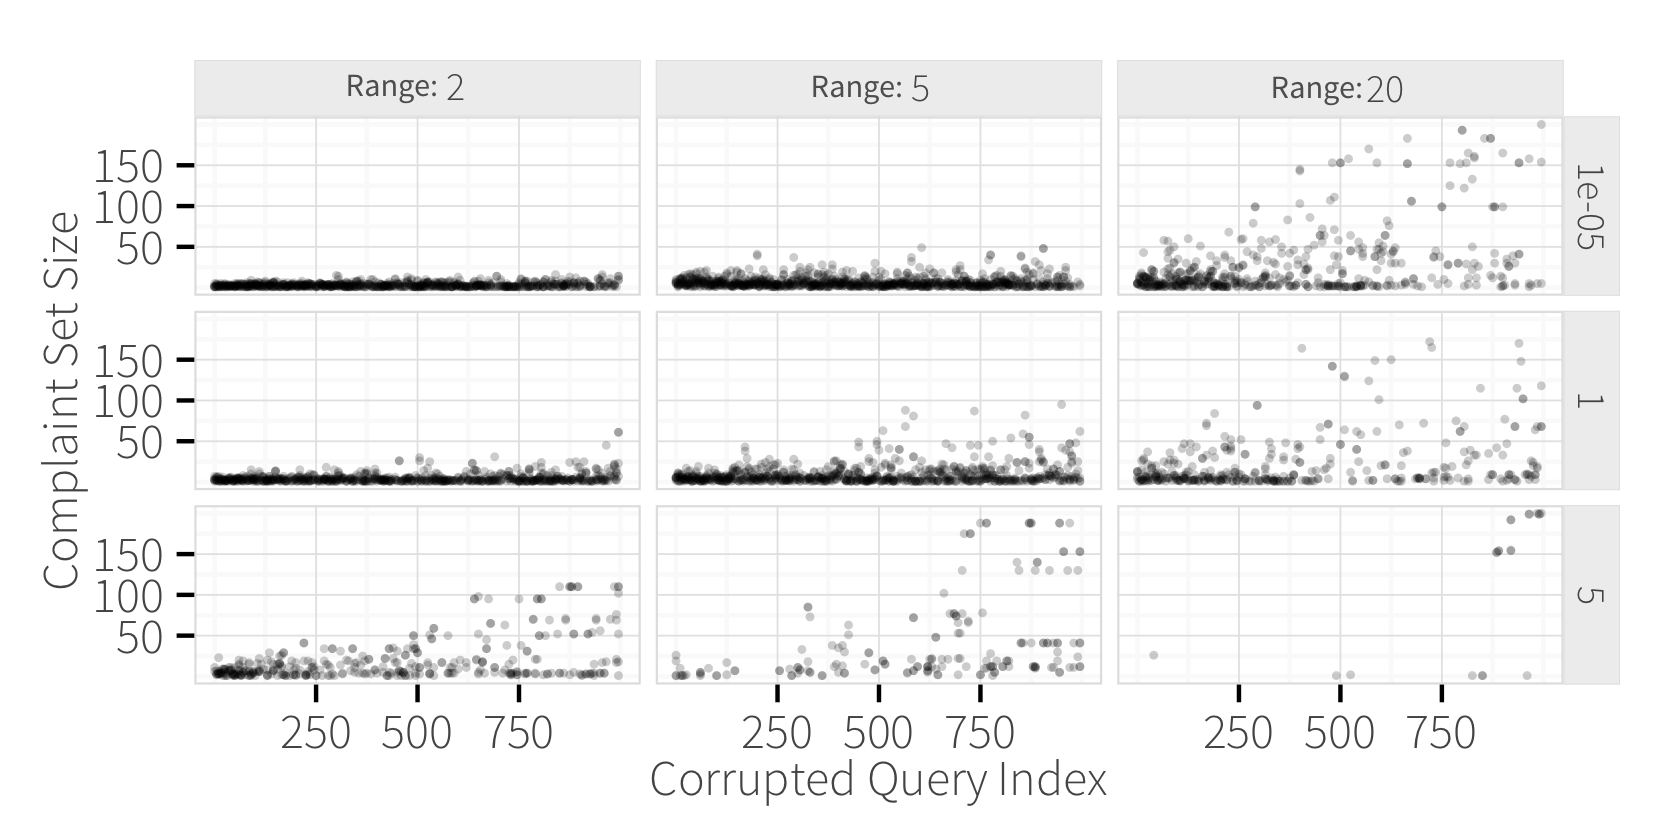
\includegraphics[width = 3in]{figures/qidxsimulation/qidx_v_ncomplaints_20attrs_const}
\caption{Corrupt query index, skew, range vs complaint set size for \textit{constant} \texttt{SET} clauses.}
\label{f:qidx_v_ncomplaints_const} 
\end{figure}

\smallskip
\emph{Constant \texttt{SET} clause: } Figure~\ref{f:qidx_v_ncomplaints_const} plots a representative set of parameters including corrupt query index, range, and skew. We plot one point
for each corrupted query index that results in a complaint set with at least one complaint. 
These results highlight several interesting trends:  With small update range and small skew factor (left upper corner)
the size of the complaint sets are relatively small, and their frequency is constant across the possible query indices.
However as we increase the range and skew, more recent queries are more likely to result in very large complaint sets (at times the size of the database).   
This effect is because the queries that have higher overlap of their \texttt{WHERE} clauses will set groups of tuples to the same value,
and over time, skew the distribution of tuple values to a small number of possible values. 
Thus, more recent corruptions that affect a large cluster of similar tuples will result in a large complaint set.
\ewu{This this effect an artifact of bad experiment design (of our query generation), or is it something that would always happen?  Need to address, since obvious question!}
And the possibility of query overlap increases with update range and skew as these two factors increase the likelihood that queries share the same \texttt{WHERE} and \texttt{SET} clause. 



\begin{figure}[t]
\centering
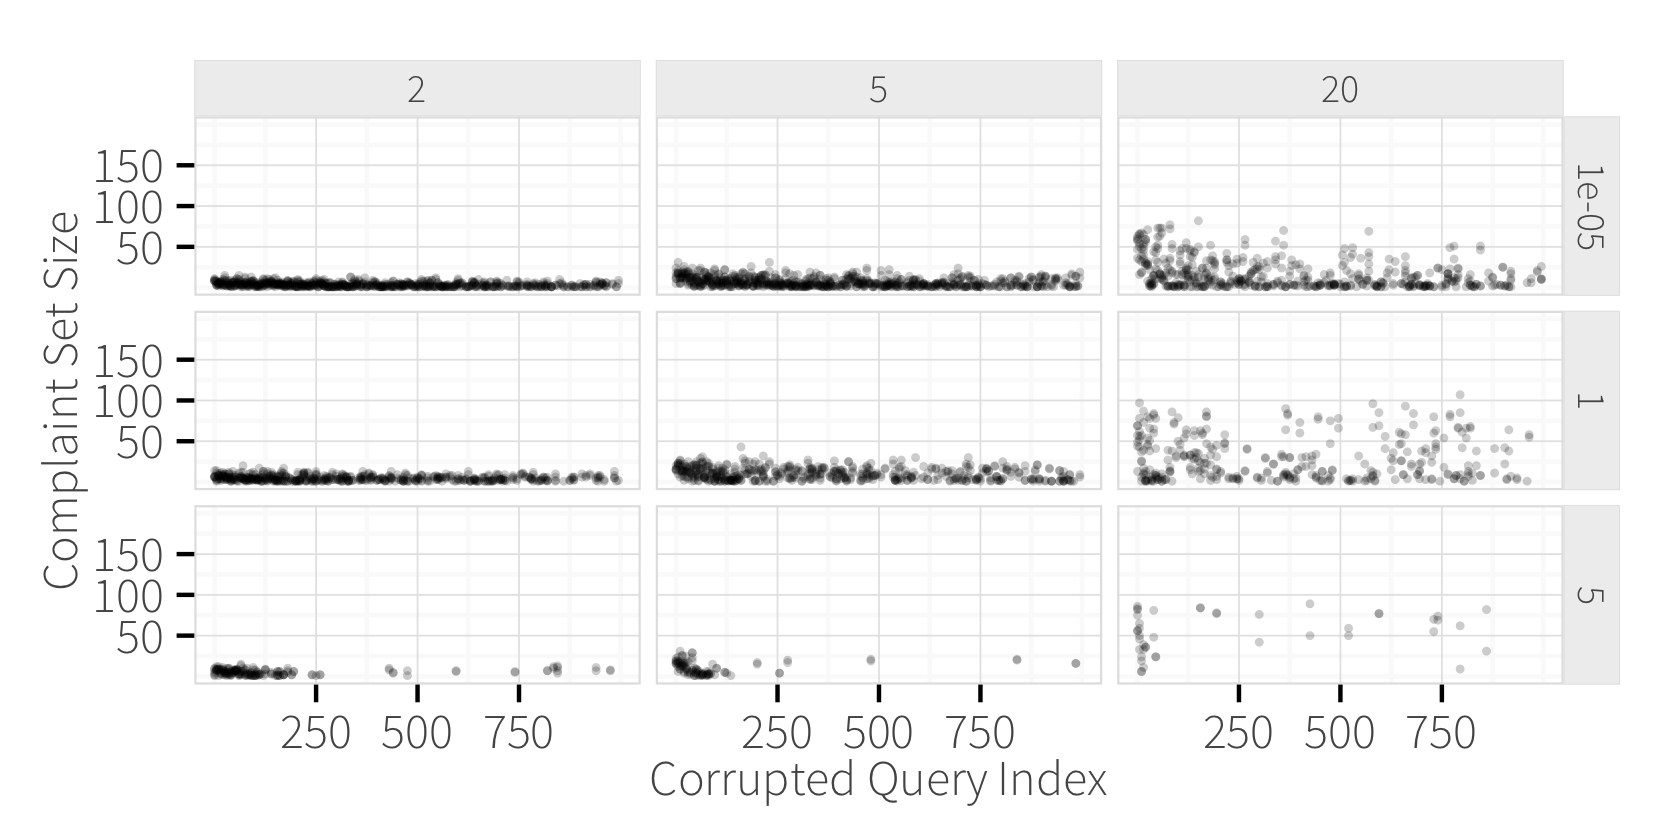
\includegraphics[width = 3in]{figures/qidxsimulation/qidx_v_ncomplaints_20attrs_rel}
\caption{Query index vs complaint set size for $set = rel$.}
\label{f:qidx_v_ncomplaints_rel} 
\end{figure}

\smallskip
\emph{Relative \texttt{SET} clause: } \xlw{In contrast to \textit{constant} \texttt{SET} queries, Figure~\ref{f:qidx_v_ncomplaints_rel} executes the 
same experiment using \textit{relative} \texttt{SET} queries.  In this setting, we find that the trend is
reversed, and older corruptions tend to result in larger complaint sets.  This is because,
subsequent \texttt{UPDATE} queries increment or decrement the attribute value, rather than
overwriting it with a constant value.  The clustering of data values due to query overlap
then increases the number of other tuples affected.
}

\fi

